\section{Related Work}
\label{sec:related}

\begin{figure*}[t]
\centering
% 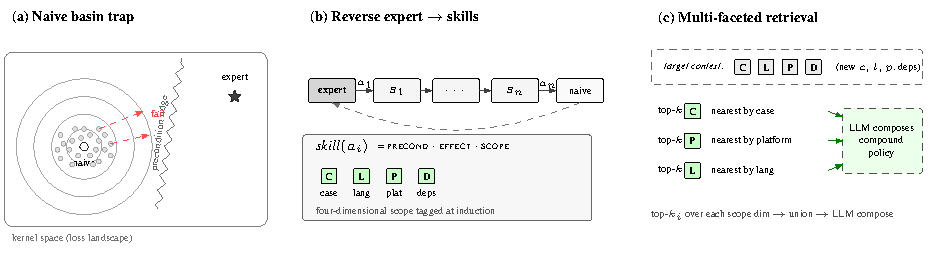
\includegraphics[width=\textwidth]{lineage-teaser.pdf}
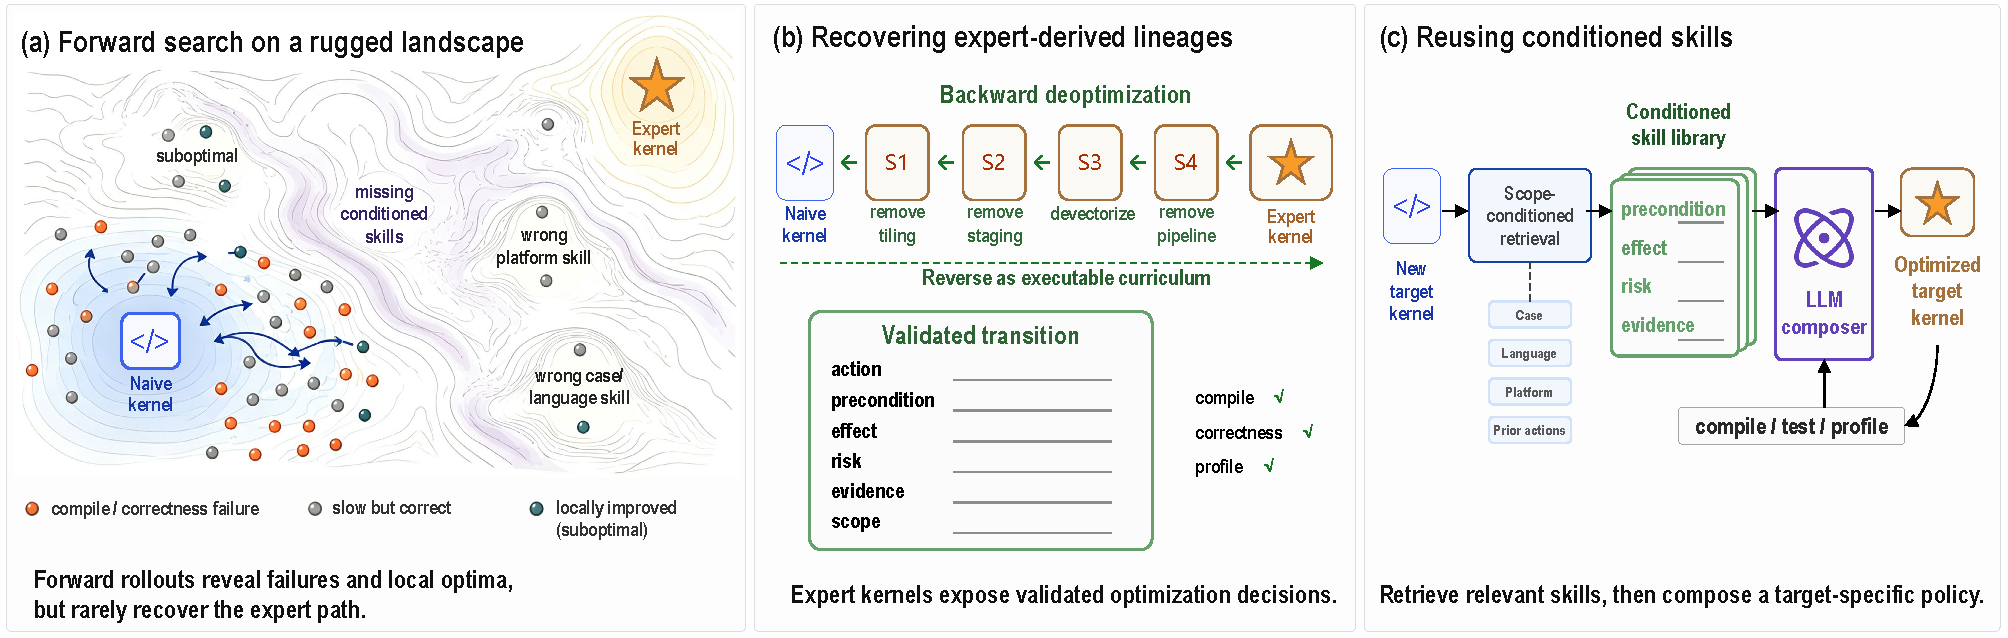
\includegraphics[width=\textwidth]{figure1.pdf}
\caption{\small
\textbf{Motivation of \sys.}
\textbf{(a)} Forward search often knows which optimizations to try but not when their preconditions hold.
\textbf{(b)} \sys walks expert kernels backward to recover validated forward transitions from simpler states toward expert states.
\textbf{(c)} The recovered skills are reused only as code-anchored candidates, with compile/test/profile gates deciding admission on new targets.
}
\label{fig:lineage-teaser}
\end{figure*}

\paragraph{LLM agents for GPU kernel optimization.}
Recent benchmarks such as KernelBench~\cite{kernelbench}, TritonBench~\cite{tritonbench}, and production-oriented FastKernels~\citep{fastkernels}, together with kernel substrates such as ThunderKittens~\cite{thunderkittens}, have made GPU-kernel generation a common testbed for LLM agents. Recent systems improve kernels through compiler/profile feedback, multi-agent refinement, DSL or minimal-program interfaces, static-analysis guidance, post-training, and search over CUDA, Triton, CuTe/CUTLASS-style, and related surfaces~\citep{gpu_kernel_scientist,geak,sakana_cuda_engineer,qimeng_kernel,astra,cutegen,tritonforge,hari2026improving,chu2025gpu,qu2026two,lou2024automatic,keet,kevin_rl_kernel,cuda_l1,autotriton}. KernelFoundry~\citep{kernelfoundry}, for example, uses quality-diversity search, prompt evolution, and template tuning to explore kernels under hardware profiling feedback, while AKO4ALL~\citep{ako4all} drives an agent through a fixed optimization protocol and Atrex Kernel Agent~\citep{atrex} works a profile-driven loop over operators sampled from production inference traces. These systems establish realistic compile/profile loops, but they largely acquire optimization knowledge by moving forward from an initial program.

\paragraph{Reusable experience and memory.}
Closest to our work are kernel agents that reuse optimization experience: AdaExplore~\cite{adaexplore} converts failures into textual rules; AccelOpt~\citep{accelopt} summarizes a run's evolving state; K-Search~\citep{ksearch} co-evolves kernels with an intrinsic world model; KernelSkill~\cite{kernel_skill} organizes expert-written skills; and KernelBlaster~\citep{kernelblaster} stores forward-rollout experience in a profile-centric memory. CuBridge~\citep{cubridge} is also related in using LLMs to understand and reconstruct expert attention kernels. \sys differs in how the memory is constructed and represented: to our knowledge, it is the first LLM-kernel memory construction method that automatically derives reusable lineages by deoptimizing expert implementations, and each skill records code/IR anchors, carriers, preconditions, effects, risks, evidence, and scope rather than only a forward trace, textual rule, or pre-existing snippet.
